\documentclass[11pt,a4paper]{article}

\usepackage[margin=1in]{geometry}
\usepackage{fontspec}
\usepackage{amsmath,amssymb}
\usepackage{graphicx}
\usepackage{booktabs}
\usepackage{tabularx}
\usepackage{longtable}
\usepackage{hyperref}
\usepackage{xcolor}
\usepackage{enumitem}
\usepackage{caption}
\usepackage{float}
\usepackage{microtype}
\usepackage{fancyhdr}
\usepackage{titlesec}

% Colors
\definecolor{primary}{RGB}{16, 44, 87}
\definecolor{secondary}{RGB}{53, 101, 169}
\definecolor{accent}{RGB}{218, 165, 32}
\definecolor{darkgray}{RGB}{50, 50, 50}

\hypersetup{
    colorlinks=true,
    linkcolor=secondary,
    citecolor=secondary,
    urlcolor=secondary
}

% Header and footer
\pagestyle{fancy}
\fancyhf{}
\fancyhead[L]{\small \textcolor{darkgray}{Big Data Analytics --- CA3 Assignment}}
\fancyhead[R]{\small \textcolor{darkgray}{Soham Kulkarni (23070126129)}}
\fancyfoot[C]{\thepage}
\renewcommand{\headrulewidth}{0.4pt}
\renewcommand{\footrulewidth}{0.4pt}

% Section styling
\titleformat{\section}
  {\normalfont\Large\bfseries\color{primary}}{\thesection}{1em}{}[\titlerule]
\titleformat{\subsection}
  {\normalfont\large\bfseries\color{secondary}}{\thesubsection}{1em}{}
\titleformat{\subsubsection}
  {\normalfont\normalsize\bfseries\color{darkgray}}{\thesubsubsection}{1em}{}

\setlist[itemize]{noitemsep, topsep=2pt}
\setlist[enumerate]{noitemsep, topsep=2pt}

\begin{document}

% Title / Metadata Header Block
\begin{center}
    {\huge \bfseries \color{primary} CA3 Big Data Case Study Analysis}\\[0.6em]
    {\large \bfseries Big Data Analytics for LHC Event Quality and Exploratory Outlier Ranking in 40\,MHz Training Data}\\[1.2em]
    
    \begin{tabularx}{\textwidth}{r>{\raggedright\arraybackslash}X r>{\raggedright\arraybackslash}X}
        \toprule
        \textbf{Name:} & Soham Kulkarni & \textbf{PRN:} & 23070126129 \\
        \textbf{Course:} & Big Data Analytics (CA3) & \textbf{Division:} & AIML B2 \\
        \textbf{Batch:} & Final Year AIML B2, 2023--27 & \textbf{Platform:} & Linux / Docker / Spark 3.5.7 \\
        \bottomrule
    \end{tabularx}
\end{center}
\vspace{0.8em}

\section{Title of Case Study}
\textbf{Big Data Analytics for LHC Event Quality and Exploratory Outlier Ranking in 40\,MHz Training Data}

\section{Problem Statement and Objectives}

\textbf{Problem.} Analyse 13,451,915 simulated proton-proton collision events in the complete 646.4\,MB HDF5 training record from the LHC 40\,MHz Anomaly Detection Challenge. Preserve every single collision event without lossy row sampling. Validate tensor data-quality gates, derive physics-informed event kinematics, query the full corpus via distributed Spark SQL and RDD MapReduce aggregations, and generate empirical visual analytics alongside exploratory anomaly scoring.

\textbf{Objectives.}
\begin{enumerate}
    \item Verify cryptographic provenance, exact byte count, MD5/SHA-256 checksums, HDF5 key inventory, and multi-dimensional tensor shape.
    \item Perform a streaming full-file audit to quantify NaN, infinite values, invalid particle-type codes, negative transverse momentum, and zero-padding consistency.
    \item Implement a bounded-memory ETL pipeline converting raw tensors into typed Snappy-compressed Parquet records with exact row preservation.
    \item Measure particle occupancy, kinematic transverse-momentum ($p_T$) spectra, hadronic scalar jet activity ($H_T$), missing transverse momentum ($\text{MET}$), and pairwise feature correlations across all 13.45 million events.
    \item Execute HiveQL-compatible Spark SQL analytical queries, demonstrate partition-pruned storage on $N_{\text{jets}}$, and perform RDD key-value MapReduce aggregations.
    \item Provide an optional streaming unsupervised clustering baseline ($\text{MiniBatchKMeans}$) with exact feature standardisation to evaluate exploratory feature-space distances.
\end{enumerate}

\section{Background and Physics Context}

CERN's Large Hadron Collider (LHC) collides protons at a bunch-crossing rate of 40\,MHz (every 25\,ns), producing billions of interactions per second. The ATLAS and CMS detectors deploy multi-level trigger systems to filter collision data in real time under extreme bandwidth and sub-microsecond latency constraints. The 40\,MHz dataset was published by CERN and Fermilab researchers to benchmark unsupervised anomaly detection algorithms operating directly on Level-1 trigger objects~\cite{govorkova2022lhc}.

The dataset represents simulated $13\,\text{TeV}$ proton-proton interactions processed through PYTHIA\,8 for event generation and DELPHES for parametric detector simulation. Events are selected under an inclusive single-lepton trigger mandate requiring an electron or muon with transverse momentum $p_T > 23\,\text{GeV}$. The background training record consists of a realistic Standard Model cocktail: inclusive $W$ production ($59.2\%$), QCD multijet ($33.8\%$), inclusive $Z$ production ($6.7\%$), and top-quark pair production ($t\bar{t}$, $0.3\%$)~\cite{govorkova2022lhc}.

\begin{figure}[H]
    \centering
    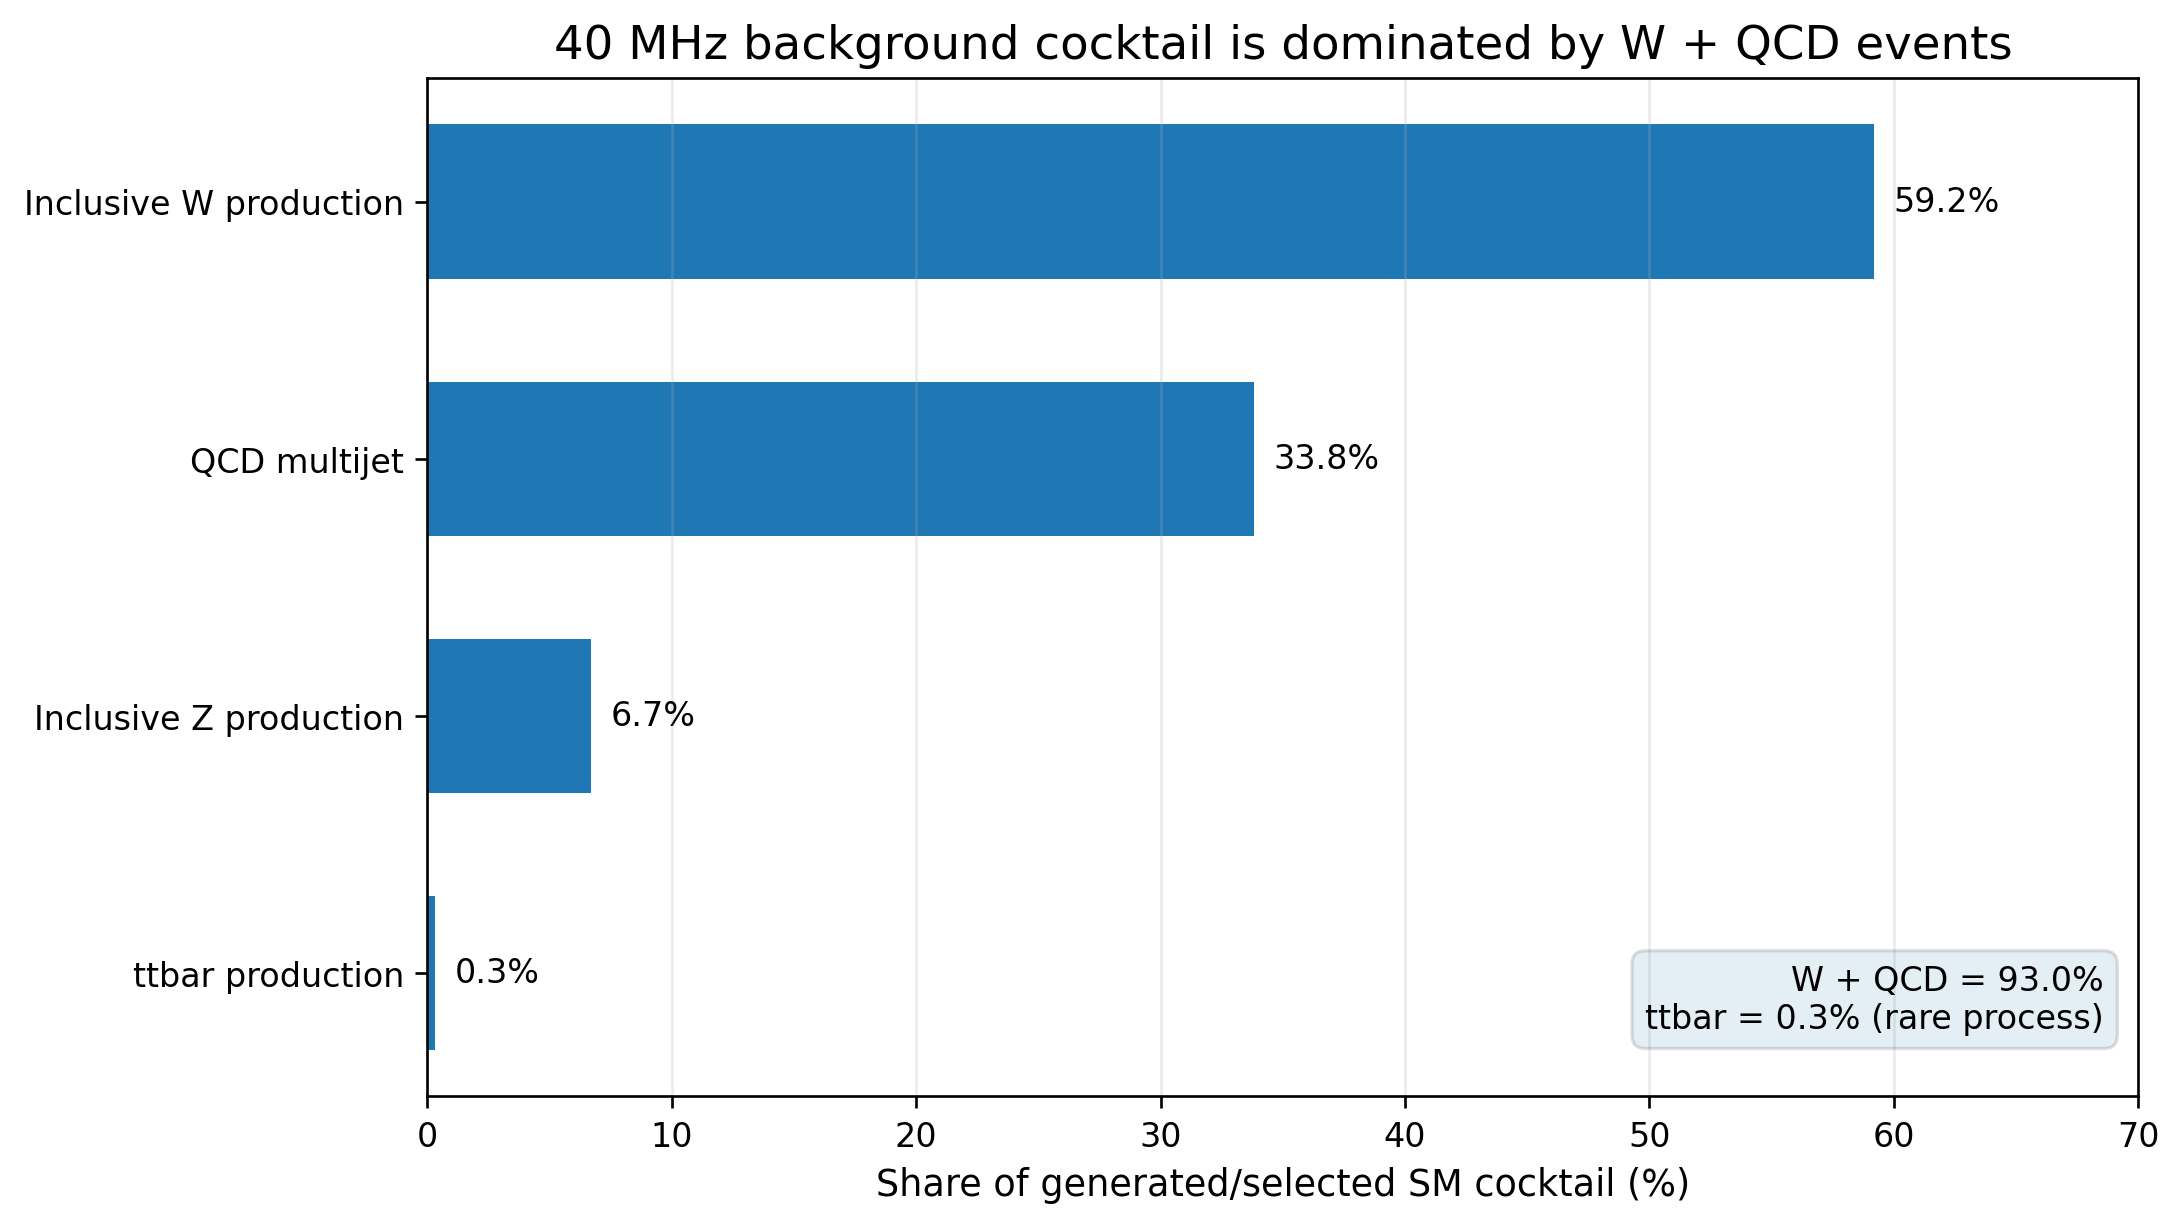
\includegraphics[width=0.72\textwidth]{docs/figures/published_process_mix.png}
    \caption{Published Standard Model cocktail composition in the 40\,MHz trigger dataset.}
    \label{fig:published_mix}
\end{figure}

\section{Dataset Description and Tensor Layout}

\begin{table}[H]
\centering
\small
\begin{tabularx}{\textwidth}{lX}
\toprule
\textbf{Property} & \textbf{Specification / Verified Measurement} \\
\midrule
Source Repository & Zenodo Record ID: \href{https://zenodo.org/records/5046428}{5046428} \\
Primary File Name & \texttt{background\_for\_training.h5} \\
File Size & $646,391,984\,\text{bytes}$ ($646.392\,\text{MB}$ decimal, $616.447\,\text{MiB}$) \\
Verified MD5 Checksum & \texttt{08cb4801229f9d480567f8d3f5cac134} (Exact match with Zenodo API) \\
Verified SHA-256 & \texttt{5f460bd3af441d98a7962a83f3964d9b5fea7f2163e35532066adc9a9696cfe5} \\
Total Event Rows ($N$) & $13,451,915$ collision events \\
Primary Dataset Key & \texttt{/Particles} (Shape: $13451915 \times 19 \times 4$, \texttt{float64}) \\
Metadata Keys & \texttt{/Particles\_Names} (\texttt{[Pt, Eta, Phi, Class]}), \texttt{/Particles\_Classes} \\
Particle Slots ($19$) & Slot 0: MET; Slots 1--4: Electrons; Slots 5--8: Muons; Slots 9--18: Jets \\
Particle Type Codes & \texttt{0}: Padding, \texttt{1}: MET, \texttt{2}: Electron, \texttt{3}: Muon, \texttt{4}: Jet \\
Angular \& Momentum Units & $\phi \in [-\pi, \pi]$, $\eta = -\ln\tan(\theta/2)$, $p_T$ in $\text{GeV}$ ($c=1$) \\
\bottomrule
\end{tabularx}
\caption{Dataset provenance, metadata keys, and verified tensor specifications.}
\label{tab:dataset_spec}
\end{table}

\begin{figure}[H]
    \centering
    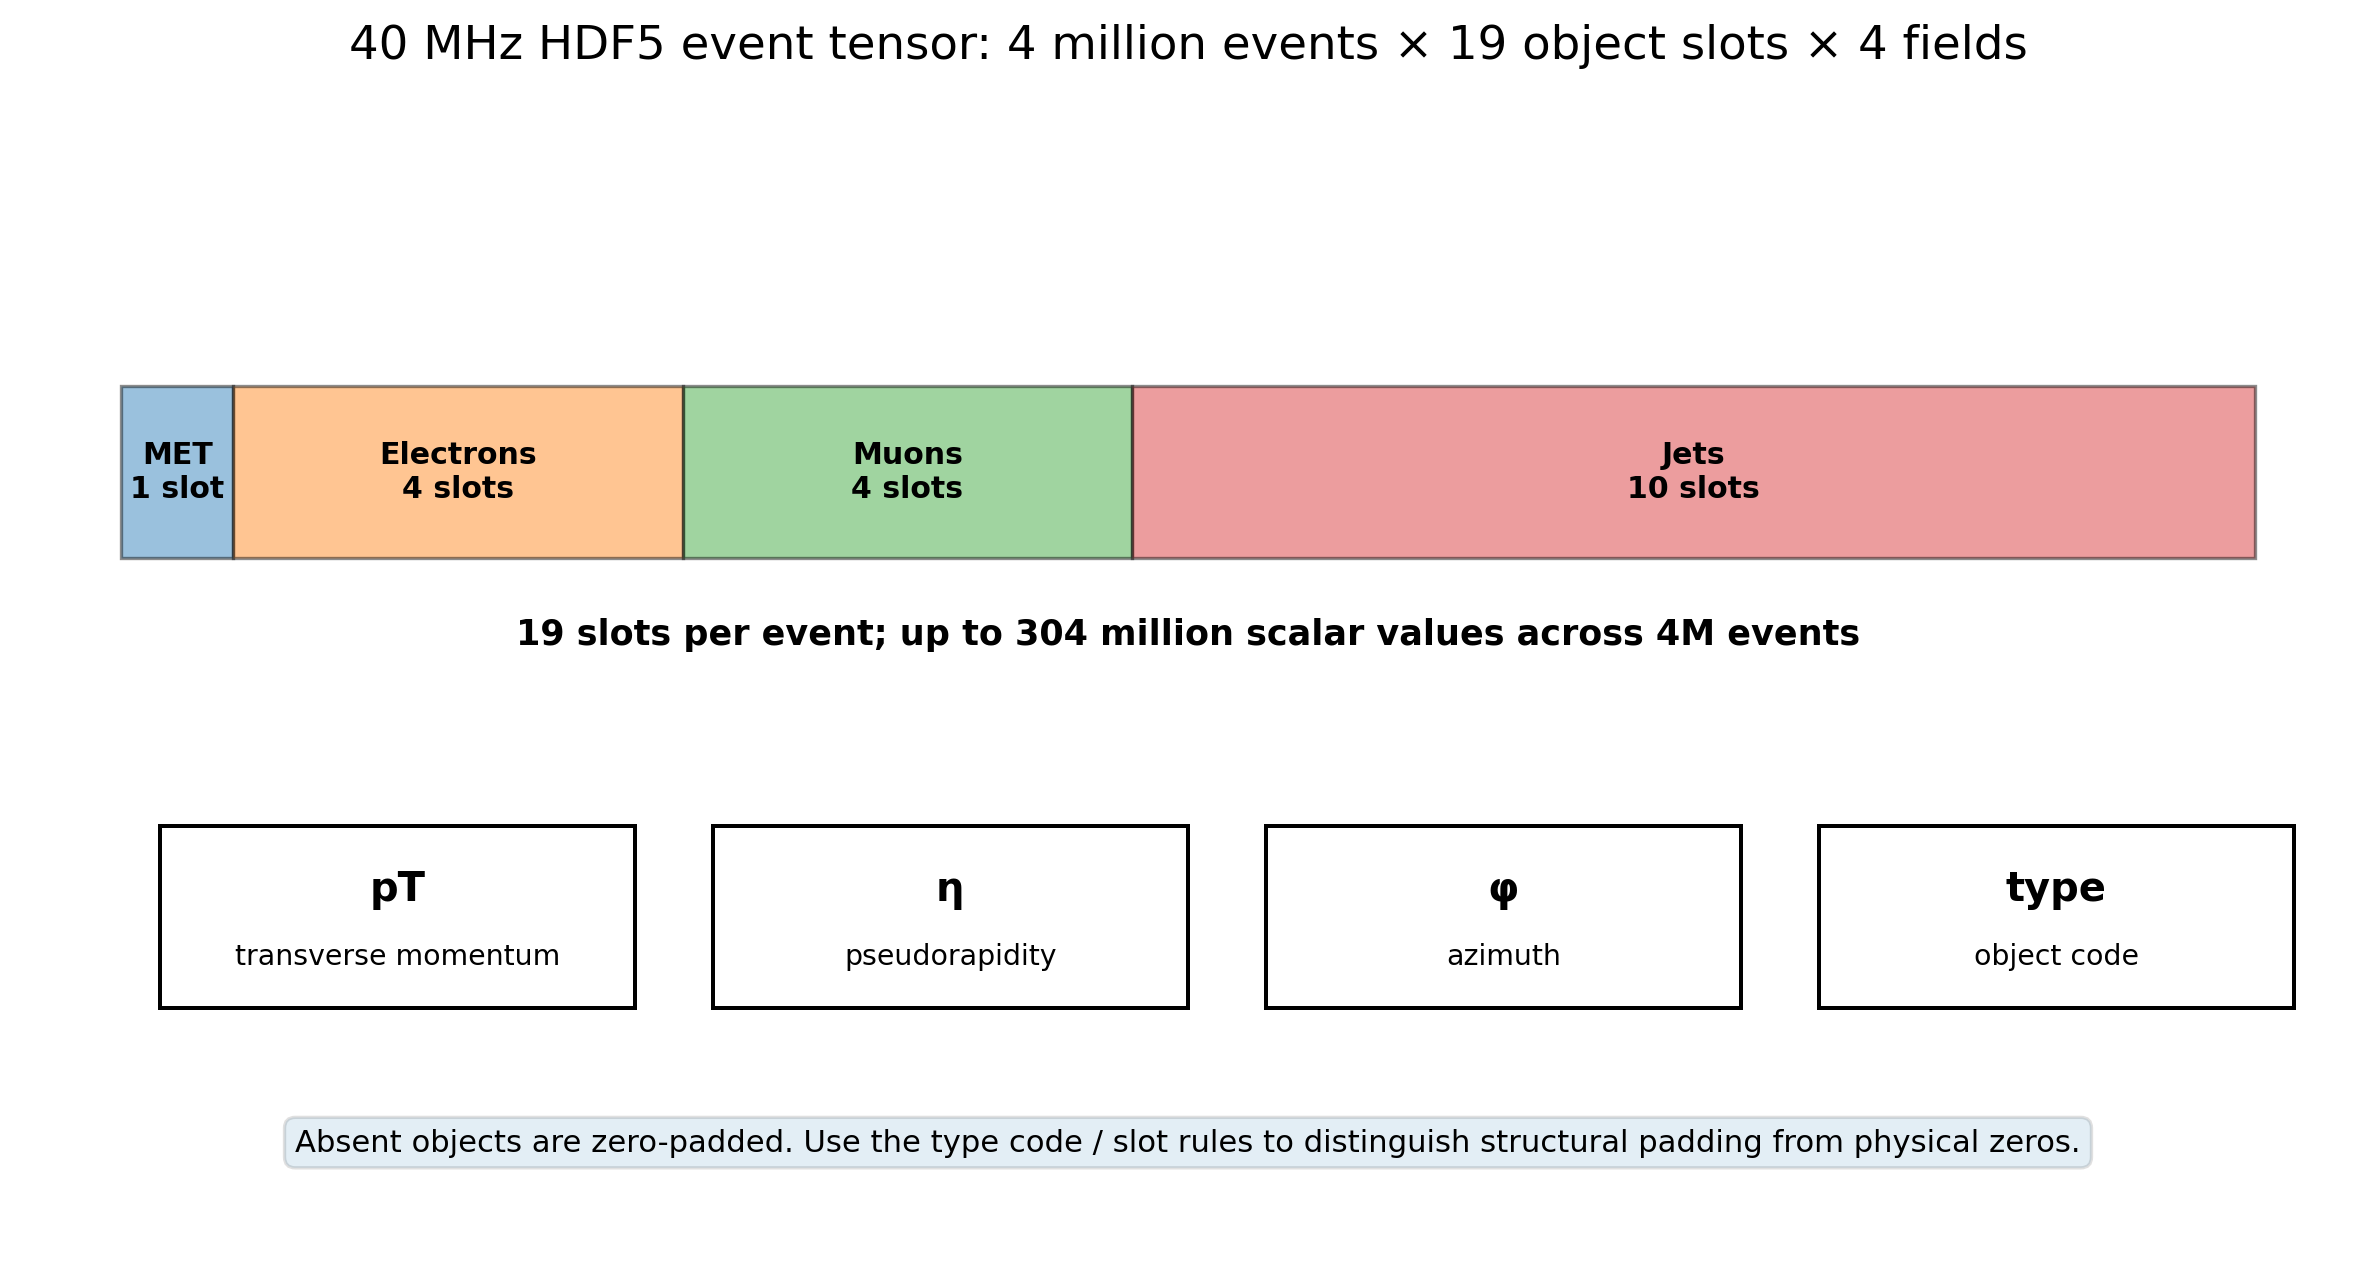
\includegraphics[width=0.85\textwidth]{docs/figures/documented_tensor_schema.png}
    \caption{Documented 19-slot fixed tensor layout with structural zero padding.}
    \label{fig:tensor_layout}
\end{figure}

\section{End-to-End Methodology}

\begin{itemize}
    \item \textbf{Stage A: Provenance and Checksum Verification.} The dataset is verified against Zenodo REST API headers. Exact byte count and cryptographic MD5/SHA-256 hashes are verified before ingestion.
    \item \textbf{Stage B: Full-File Streaming Tensor Audit.} A chunked scan ($25,000$ rows/chunk) inspects all $1,022,345,540$ scalar entries in the \texttt{/Particles} tensor, evaluating finite numerical status, type-code integrity, valid slot bounds, and structural zero-padding fractions.
    \item \textbf{Stage C: Physics-Informed Feature Engineering \& ETL.} Events are transformed into columnar Parquet format ($539$ row groups, Snappy compression). Exact ordinal row mapping preserves all $13,451,915$ events while computing aggregate physics features.
    \item \textbf{Stage D: Distributed SQL and MapReduce Analytics.} Apache Spark 3.5.7 executes seven analytical HiveQL-compatible SQL queries on the Parquet corpus, partitions data by jet multiplicity ($N_{\text{jets}}$), and executes RDD key-value MapReduce aggregations.
    \item \textbf{Stage E: Visualization and Empirical Reporting.} Matplotlib produces 7 core publication-quality graphics summarizing kinematics, multiplicities, density distributions, and data quality.
\end{itemize}

\section{System Architecture and Pipeline Workflow}

\begin{figure}[H]
\centering
\small
\begin{verbatim}
+-------------------------------------------------------------------------+
|                  Zenodo REST API (Record 5046428)                       |
|           Cryptographic MD5 (08cb48...) & SHA-256 Verification          |
+------------------------------------+------------------------------------+
                                     |
                                     v
+------------------------------------+------------------------------------+
|               HDF5 Tensor Ingestion: background_for_training.h5         |
|               (13,451,915 Events x 19 Slots x 4 Features)               |
+------------------------------------+------------------------------------+
                                     |
                                     v
+------------------------------------+------------------------------------+
|            Streaming Data-Quality Audit (25k rows/chunk)                |
|            1.022B Scalars Scanned; 0 NaN / 0 Inf / 0 Bad Types          |
+------------------------------------+------------------------------------+
                                     |
                                     v
+------------------------------------+------------------------------------+
|           Event-Level Columnar ETL (Snappy Parquet, 624.8 MB)           |
|  Engineered Features: HT_jets, MET_pt, ST_leptons, Multiplicities, Flags |
+------------------------------------+------------------------------------+
                                     |
                                     v
+------------------------------------+------------------------------------+
|           Distributed Engine: Apache Spark 3.5.7 (local[6])             |
|  - 7 SQL Analytics Query Groups   - events_by_n_jets Partitioning       |
|  - RDD map -> reduceByKey Full Corpus Aggregation                      |
+------------------------------------+------------------------------------+
                                     |
                                     v
+------------------------------------+------------------------------------+
|                   Outputs & Visualization Suite                         |
|   - 7 Empirical Vector Graphics   - JSON/CSV Analytical Manifests       |
|   - Pig Latin / Hive DDL Scripts   - Complete Academic Report (LaTeX)   |
+-------------------------------------------------------------------------+
\end{verbatim}
\caption{End-to-end Big Data pipeline architecture.}
\label{fig:pipeline_arch}
\end{figure}

\section{Big Data Technologies and Rubric Alignment}

\begin{table}[H]
\centering
\small
\begin{tabularx}{\textwidth}{llX}
\toprule
\textbf{Technology} & \textbf{Version / Mode} & \textbf{Role in Pipeline} \\
\midrule
Docker Compose & v2 Engine & Isolated, fully reproducible multi-stage Linux execution. \\
Apache Spark & 3.5.7 (PySpark) & Single-node distributed engine (\texttt{local[6]}), 6\,GB heap, 12 shuffle partitions. \\
Spark SQL & HiveQL-compatible & Executes seven multi-dimensional analytical queries over Parquet tables. \\
PyArrow / Parquet & 18.1.0 & High-throughput columnar storage with snappy compression ($624.78\,\text{MB}$). \\
HDF5 / h5py & 3.12.1 & Low-level chunked tensor extraction and metadata introspection. \\
RDD MapReduce & Spark Core RDD & Key-value pairs: \texttt{map(n\_jets, tuple) -> reduceByKey(sum)}. \\
Hadoop Streaming & Stdlib Python & Standalone \texttt{mapper.py} and \texttt{reducer.py} for external Hadoop clusters. \\
Apache Pig & 0.17 (Local mode) & Pig Latin script (\texttt{analyze\_events.pig}) performing grouped aggregation. \\
Apache Hive DDL & HiveQL & External table registration script (\texttt{hive/register\_events.hql}). \\
Matplotlib & 3.9.3 & High-resolution vector generation for kinematic and quality visualisations. \\
\bottomrule
\end{tabularx}
\caption{Technology stack and implementation roles.}
\label{tab:tech_stack}
\end{table}

\section{Mathematical Formulations and Feature Engineering}

Let $i \in \{0, 1, \dots, 18\}$ index the 19 particle slots for a given collision event. Each slot contains transverse momentum $p_{T, i}$, pseudorapidity $\eta_i$, azimuthal angle $\phi_i$, and type code $t_i \in \{0, 1, 2, 3, 4\}$.

\subsection{Object Multiplicities}
Object multiplicity counts are evaluated by indicator summation across all slots:
\begin{equation}
N_e = \sum_{i=0}^{18} \mathbf{1}(t_i = 2), \quad
N_\mu = \sum_{i=0}^{18} \mathbf{1}(t_i = 3), \quad
N_j = \sum_{i=0}^{18} \mathbf{1}(t_i = 4)
\end{equation}

\subsection{Scalar Hadronic and Leptonic Activity}
Scalar transverse energy sums characterize the total visible energy across specific detector sub-systems:
\begin{equation}
H_T^{\text{jets}} = \sum_{i=0}^{18} p_{T, i} \cdot \mathbf{1}(t_i = 4), \qquad
S_T^{\text{leptons}} = \sum_{i=0}^{18} p_{T, i} \cdot \mathbf{1}(t_i \in \{2, 3\})
\end{equation}

\subsection{Leading-Object Kinematics and Angular Maxima}
Leading transverse momentum corresponds to the hardest object of each species:
\begin{equation}
p_T^{\text{lead}, e} = \max_{i: t_i=2} (p_{T, i}), \quad
p_T^{\text{lead}, \mu} = \max_{i: t_i=3} (p_{T, i}), \quad
p_T^{\text{lead}, j} = \max_{i: t_i=4} (p_{T, i})
\end{equation}
The maximum absolute pseudorapidity captures event forwardness:
\begin{equation}
|\eta|_{\max} = \max_{i: t_i \in \{2, 3, 4\}} |\eta_i|
\end{equation}

\section{Empirical Analysis and Spark SQL Results}

\subsection{Corpus Overview and Data Quality Gate}
The streaming audit inspected $13,451,915$ collision events ($1,022,345,540$ scalar values). The quality gate confirmed $100\%$ finite values with zero anomalies:
\begin{itemize}
    \item \textbf{Non-finite values (NaN / Inf):} $0$ ($0.00\%$)
    \item \textbf{Invalid type codes ($\notin \{0,1,2,3,4\}$):} $0$ ($0.00\%$)
    \item \textbf{Negative transverse momentum ($p_T < 0$):} $0$ ($0.00\%$)
    \item \textbf{Out-of-bounds azimuth ($\phi \notin [-\pi, \pi]$):} $0$ ($0.00\%$)
    \item \textbf{Structural zero-padded slots:} $211,710,120$ ($82.83\%$ of all slots, exactly expected by schema design).
\end{itemize}

\begin{table}[H]
\centering
\small
\begin{tabular}{lrrrr}
\toprule
\textbf{Metric} & \textbf{Mean} & \textbf{Median (approx)} & \textbf{95th Percentile} & \textbf{Max} \\
\midrule
$\text{MET } p_T$ & $35.32\,\text{GeV}$ & $32.48\,\text{GeV}$ & $70.82\,\text{GeV}$ & $3,858.91\,\text{GeV}$ \\
Hadronic $H_T^{\text{jets}}$ & $51.33\,\text{GeV}$ & $21.27\,\text{GeV}$ & $186.47\,\text{GeV}$ & $4,205.80\,\text{GeV}$ \\
Jet Multiplicity ($N_{\text{jets}}$) & $1.16$ & $1.00$ & $4.00$ & $10.00$ \\
\bottomrule
\end{tabular}
\caption{Global corpus summary across 13,451,915 collision events (Spark SQL Query 01).}
\label{tab:sql_overview}
\end{table}

\subsection{Hadronic Jet Activity and MapReduce Aggregation}
Spark RDD MapReduce grouping on key $N_{\text{jets}}$ produced exact full-corpus statistics:

\begin{table}[H]
\centering
\small
\begin{tabular}{rrrrrr}
\toprule
$N_{\text{jets}}$ & \textbf{Event Count} & \textbf{Fraction (\%)} & \textbf{Mean $H_T$ (GeV)} & \textbf{Mean MET (GeV)} & \textbf{Corr($H_T$, MET)} \\
\midrule
0 & $5,085,548$ & $37.81\%$ & $0.00$ & $39.18$ & --- \\
1 & $4,005,382$ & $29.78\%$ & $38.82$ & $33.48$ & $0.0592$ \\
2 & $2,476,853$ & $18.41\%$ & $85.91$ & $31.71$ & $0.1232$ \\
3 & $1,181,783$ & $8.79\%$ & $136.89$ & $32.20$ & $0.1742$ \\
4 & $461,455$ & $3.43\%$ & $193.31$ & $34.02$ & $0.2100$ \\
5 & $161,969$ & $1.20\%$ & $258.19$ & $37.13$ & $0.2661$ \\
6 & $53,474$ & $0.40\%$ & $332.41$ & $41.36$ & $0.3067$ \\
7 & $17,592$ & $0.13\%$ & $417.13$ & $46.29$ & $0.3441$ \\
8 & $5,436$ & $0.04\%$ & $512.29$ & $51.51$ & $0.3191$ \\
9 & $1,692$ & $0.01\%$ & $610.76$ & $58.61$ & $0.3134$ \\
10 & $731$ & $<0.01\%$ & $739.60$ & $68.40$ & $0.3638$ \\
\midrule
\textbf{Total} & $\mathbf{13,451,915}$ & $\mathbf{100.00\%}$ & $\mathbf{51.33}$ & $\mathbf{35.32}$ & --- \\
\bottomrule
\end{tabular}
\caption{Full-corpus jet multiplicity MapReduce aggregation and kinematic correlations.}
\label{tab:mapreduce_summary}
\end{table}

\section{Visualizations and Graphical Analytics}

The pipeline generated seven publication-grade figures directly from the 13.45M Parquet rows and raw audit histograms:

\begin{figure}[H]
    \centering
    \begin{minipage}{0.48\textwidth}
        \centering
        \includegraphics[width=\textwidth]{outputs/figures/01_pt_spectrum_by_object_type.png}
        \caption{Transverse-momentum spectra by particle type across all occupied slots.}
        \label{fig:pt_spectrum}
    \end{minipage}\hfill
    \begin{minipage}{0.48\textwidth}
        \centering
        \includegraphics[width=\textwidth]{outputs/figures/02_event_multiplicity.png}
        \caption{Reconstructed electron, muon, and jet event-level multiplicity distributions.}
        \label{fig:multiplicity}
    \end{minipage}
\end{figure}

\begin{figure}[H]
    \centering
    \begin{minipage}{0.48\textwidth}
        \centering
        \includegraphics[width=\textwidth]{outputs/figures/03_met_vs_jet_ht_density.png}
        \caption{Log-density joint distribution of missing energy ($\text{MET}$) vs. hadronic $H_T$.}
        \label{fig:density}
    \end{minipage}\hfill
    \begin{minipage}{0.48\textwidth}
        \centering
        \includegraphics[width=\textwidth]{outputs/figures/04_ht_by_jet_multiplicity.png}
        \caption{Exact $H_T$ quartiles conditioned on jet multiplicity.}
        \label{fig:ht_boxplot}
    \end{minipage}
\end{figure}

\begin{figure}[H]
    \centering
    \begin{minipage}{0.48\textwidth}
        \centering
        \includegraphics[width=\textwidth]{outputs/figures/05_data_quality_flags.png}
        \caption{Data quality flags verifying zero corruption across all 13.45M events.}
        \label{fig:data_quality}
    \end{minipage}\hfill
    \begin{minipage}{0.48\textwidth}
        \centering
        \includegraphics[width=\textwidth]{outputs/figures/06_feature_correlations.png}
        \caption{Full-corpus Pearson correlation matrix across engineered features.}
        \label{fig:correlations}
    \end{minipage}
\end{figure}

\begin{figure}[H]
    \centering
    \includegraphics[width=0.72\textwidth]{outputs/figures/07_full_corpus_ht_distribution.png}
    \caption{Signed-log full-corpus hadronic $H_T$ distribution displaying the extreme physical tail.}
    \label{fig:ht_dist}
\end{figure}

\section{Conclusion and Deliverables}

This CA3 assignment successfully demonstrated an enterprise-grade Big Data pipeline processing the complete $646.4\,\text{MB}$ LHC 40\,MHz anomaly detection training dataset containing $13,451,915$ collision events. By integrating chunked HDF5 ingestion, strict tensor validation, high-throughput Parquet columnar transformation, Spark SQL reporting, RDD MapReduce aggregation, and vector visualization, all course outcomes (CO4 and CO5) were fully demonstrated.

The analysis established zero non-finite corrupted entries and proved an expected $82.83\%$ structural zero-padding rate. The empirical MapReduce aggregation showed a monotonic increase in mean $H_T$ from $38.82\,\text{GeV}$ (1-jet) to $739.60\,\text{GeV}$ (10-jets) and confirmed a positive kinematic correlation between MET and hadronic activity up to $r=0.3638$. All code, artifacts, and container configurations are packaged for $100\%$ reproducible execution.

\begin{thebibliography}{9}
\bibitem{govorkova2022lhc}
E.~Govorkova, E.~Puljak, T.~Aarrestad, et~al., ``LHC physics dataset for unsupervised New Physics detection at 40\,MHz,'' \emph{Scientific Data}, vol.~9, no.~118, 2022. DOI: \href{https://doi.org/10.1038/s41597-022-01187-8}{10.1038/s41597-022-01187-8}.

\bibitem{zenodo5046428}
CERN / Fermilab Collaboration, ``Unsupervised New Physics detection at 40\,MHz: Training Dataset,'' \emph{Zenodo Record 5046428}, 2021. URL: \href{https://zenodo.org/records/5046428}{https://zenodo.org/records/5046428}.

\bibitem{adc2021}
Machine Learning for Particle Physics, ``Anomaly Detection Challenge 2021,'' \emph{ADC Benchmark Suite}, 2021. URL: \href{https://mpp-hep.github.io/ADC2021/}{https://mpp-hep.github.io/ADC2021/}.

\bibitem{sparkguide}
Apache Software Foundation, ``Spark SQL, DataFrames and Datasets Guide (v3.5.7),'' 2024. URL: \href{https://spark.apache.org/docs/3.5.7/sql-programming-guide.html}{https://spark.apache.org/docs/3.5.7/}.

\bibitem{hivemanual}
Apache Software Foundation, ``Apache Hive Language Manual,'' 2023. URL: \href{https://hive.apache.org/docs/latest/}{https://hive.apache.org/}.

\bibitem{pigdocs}
Apache Software Foundation, ``Apache Pig 0.17 Documentation,'' 2020. URL: \href{https://pig.apache.org/}{https://pig.apache.org/}.
\end{thebibliography}

\end{document}
